\documentclass{article}
\usepackage[utf8]{inputenc}
\usepackage[T1]{fontenc}
\usepackage[francais]{babel}
\usepackage{listings}
\usepackage{verbatim}
\usepackage{geometry}
\usepackage{hyperref}
\usepackage{graphicx}

\geometry{
    a4paper,
    total={170mm,257mm},
    left=20mm,
    top=20mm,
}

\title{\textbf{EarlyWarning}\\Guide de Configuration}
\author{Thomas Kowalski}
\date{Juillet 2018}

\lstset{
    caption=\lstname,
    showstringspaces=false,
    showspaces=false
}

\begin{document}

\maketitle

\pagebreak
\tableofcontents

\pagebreak
\section{Fonctionnement général de l'alarme précoce}

\begin{center}
    \begin{figure}[h!]
      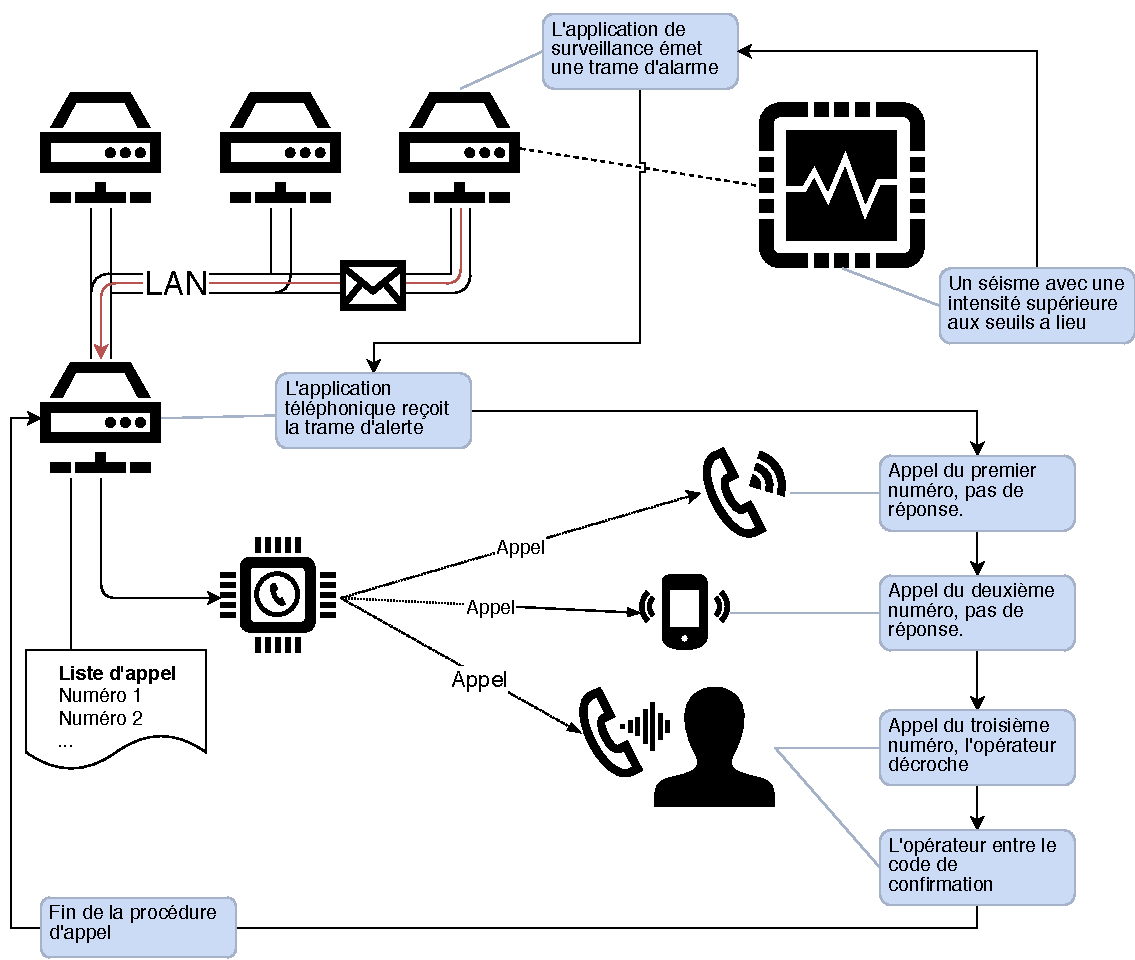
\includegraphics[width=\linewidth]{Illustrations/Fonctionnement_General.pdf}
      \caption{Schéma du fonctionnement général de l'Alarme Précoce}
      \label{fig:fonctionnement}
    \end{figure}
\end{center}

Le principe général du système d'alarme précoce est de déclencher des appels téléphoniques vocaux interactifs et de diffuser des messages d'alertes par différents modes de communication (SMS, e-mail) en fonction d'un certain nombre de déclencheurs (\emph{triggers}). \\
Un déclencheur peut être une sismicité importante, le dépassement de valeurs de seuil (\texttt{RSAM1} par exemple), une panne matérielle, logicielle ou électrique, \emph{etc.}

Les déclencheurs sont créés par des logiciels spécifiques, hébergées sur des serveurs informatiques. Les déclencheurs transitent via le réseau informatique.

Lorsqu'un déclencheur est émis, le système d'alarme précoce l'analyse. Il en tire un certain nombre d'informations : 
\begin{itemize}
    \item L'annuaire à utiliser pour les appels ;
    \item La séquence de confirmation ;
    \item La priorité du message ;
    \item Le message en lui-même ;
    \item \emph{etc.}
\end{itemize}

Commence ensuite une phase d'appel. Celle-ci se base sur la liste d'appel contenant un nombre illimité de numéros de téléphone. Le système d'alarme commence par le premier contact de la liste et initie l'appel.

L'appel émis est vocal et interactif. Le message pré-enregistré est énoncé et la personne appelée doit saisir une séquence de confirmation (suite de numéros à saisir sur le clavier de son téléphone) pour valider la réception du message.

Tant que la séquence de validation n'a pas été enregistrée ou l'appel décroché, l'application va continuer d'appeler les numéros présents dans son annuaire. La phase d'appel laisse sonner un nombre maximum de fois avant d'abandonner un appel. Elle détermine lorsqu'un répondeur prend l'appel et abandonne l'appel. Elle raccroche tout appel décroché au bout d'un certain délai, que l'utilisateur ait ou non entré la séquence de confirmation (pour libérer la ligne et passer à l'appel suivant).\\

De plus, si la passerelle téléphonique par défaut (Asterisk) est inaccessible, l'application peut également utiliser une alarme anti-intrusion (module \emph{Charon I}) comme passerelle téléphonique pour émettre une alerte d'urgence.\\

Enfin, l'application intègre différents outils, notamment une interface Web d'édition d'annuaires, un logiciel d'envoi de \emph{triggers} permettant la vérification du bon fonctionnement du système.

\pagebreak
\section{Introduction et remarques générales}

\subsection{Arguments de la ligne de commande pour EarlyWarning}

\begin{description}
    % \item[\texttt{--novalidation}] Désactive la vérification de la configuration au démarrage ;
    \item[\texttt{--testcall}] Créé et ajoute à la pile un \emph{trigger} afin de vérifier le bon fonctionnement de la passerelle téléphonique ;
    \item[\texttt{--testcalls}] Créé et ajoute à la pile deux \emph{triggers} afin de vérifier le fonctionnement de la passerelle téléphonique ;
    \item[\texttt{--searchresources}] Cherche automatiquement dans les sous dossiers du dossier actuel (\emph{working directory}) le dossier où se trouve la configuration. Utile avant tout lors du débogage, pour tester une nouvelle version sans avoir à la déplacer dans le dossier où se trouvent les ressources.
\end{description}

\subsection{Commandes de redémarrage}

Toute modification de la configuration d'Asterisk ou de la configuration d'EarlyWarning demande un redémarrage des applications concernées. 

\begin{description}
    \item[Asterisk] Utiliser la commande \texttt{service asterisk restart}, le redémarrage est immédiat ;
    \item[EarlyWarning] Utiliser la commande \texttt{systemctl restart earlywarning.service}.
\end{description}

\paragraph{Attention} Le téléchargement des dépendances peut prendre beaucoup de temps après la réinitialisation.

\pagebreak
\section{Installations des pré-requis}

\subsection{Installation de Git}

Git s'installe facilement avec Aptitude :

\begin{verbatim}
    apt-get install git
\end{verbatim}

\subsection{Installation de Java}

Sous Debian, on utilisera l'OpenJDK dans sa dernière version disponible.

\paragraph{Exemple avec la version 8}

\begin{verbatim}
    apt-get install openjdk-8-jdk
\end{verbatim}

L'installation du \textbf{JDK} est nécessaire pour pouvoir compiler l'application. Le \textbf{JRE} ne suffit pas.

\paragraph{Remarque} La nouvelle version de l'alarme précoce est conçue pour fonctionner avec Java à partir de sa version 7.

\subsection{Installation d'Asterisk}

Asterisk s'installe facilement avec Aptitude :

\begin{verbatim}
    sudo apt-get install asterisk
\end{verbatim}

\subsection{Installation de Maven}

Le projet utilise la technologie Maven, que l'on peut installer avec Aptitude :

\begin{verbatim}
    apt-get install maven
\end{verbatim}

\subsection{Récupération des sources de l'application}

Les sources se récupèrent depuis le dépôt Git avec la commande \texttt{clone}

\begin{verbatim}
    git clone https://github.com/kowalskithomas/alarmeprecoceovpf.git
\end{verbatim}

\subsection{Réinitialisation du dépôt Maven local}

Dans de rares cas, des problèmes de compilation peuvent survenir avec Maven. La réinitialisation du dépôt local peut résoudre ces problèmes.

\begin{verbatim}
    rm -rf ~/.m2
\end{verbatim}

\pagebreak
\section{Compilation d'EarlyWarning}

EarlyWarning utilise \hyperlink{https://maven.apache.org}{Maven}     pour la gestion des dépendances, les tests unitaires, la compilation et le \emph{packaging}.

Cette section couvre ces différents aspects. 

\paragraph{Remarque} Les commandes Maven doivent être exécutées depuis le dossier \texttt{java} qui contient le dossier \texttt{src} et le fichier \texttt{pom.xml}.

\subsection{Lecture et installation des dépendances}

Grâce au fichier \texttt{pom.xml} présent dans le code source, Maven peut déterminer l'arbre des dépendances de l'artefact EarlyWarning. \\

EarlyWarning utilise deux types de dépendances :

\begin{itemize}
    \item Des dépendances libres (\emph{Apache Commons}, \emph{LF4J}) ;
    \item Des dépendances propriétaires ou internes. 
\end{itemize}

Les premières peuvent directement être récupérées et installées par Maven depuis le Maven Repository dans le \emph{local Maven repository}.

Les secondes doivent cependant être installées par Maven depuis des archives JAR fournies avec le code source. Cette installation se fait grâce au \emph{plugin} \texttt{maven-install}. \\

Pour installer les dépendances (libres et propriétaires), utiliser la commande 

\begin{verbatim}
    mvn validate
\end{verbatim}

Le déroulement de cette commande peut prendre un certain temps, notamment si le dépôt Maven local est vierge. En effet, toutes les dépendances doivent alors être téléchargées.

\subsection{Tests unitaires}

Maven permet de lancer directement les tests unitaires. Pour cela, utiliser la commande suivante :

\begin{verbatim}
    mvn clean test
\end{verbatim}

\paragraph{Remarque} Lors de la première exécution des tests, le téléchargement de dépendances aditionnelles sera nécessaire.

\paragraph{Remarque} \texttt{mvn clean} permet de supprimer les binaires existants et de forcer une recompilation de l'ensemble des sources.

La sortie finale est censée ressembler à 

\begin{verbatim}
[INFO] Results:
[INFO] 
[INFO] Tests run: 25, Failures: 0, Errors: 0, Skipped: 0
[INFO] 
[INFO] ------------------------------------------------------------------------
[INFO] BUILD SUCCESS
[INFO] ------------------------------------------------------------------------
[INFO] Total time: 11.501s
[INFO] Finished at: Tue Jul 17 06:09:57 UTC 2018
[INFO] Final Memory: 14M/36M
[INFO] ------------------------------------------------------------------------
\end{verbatim}


\subsection{Compilation}

Pour compiler l'ensemble des classes, utiliser 

\begin{verbatim}
    mvn clean compile
\end{verbatim}

\subsection{\emph{Packaging} (en utilisant Maven)}

Enfin, pour créer une archive Java (JAR) du projet EarlyWarning, utiliser

\begin{verbatim}
    mvn package
\end{verbatim}

Le fichier \texttt{pom.xml} est configuré pour que l'étape de \texttt{packaging} utilise le \emph{plugin} Maven \emph{shadow}. Celui-ci permet d'inclure dans le JAR final toutes les dépendances du projet.

Ainsi, lors du déploiement, seul le fichier généré \texttt{AlarmePrecoce-x.x.x.jar} est nécessaire à l'exécution de l'application.

Les ressources ne sont, quant à elles, pas incluses dans le JAR et doivent donc être copiées dans le même dossier où le JAR est déployé.

\begin{verbatim}
-rw-r--r--  1 root root 5382533 Jul 17 06:13 AlarmePrecoce-1.0.1.jar
-rw-r--r--  1 root root    5508 Jul 17 06:13 dependency-reduced-pom.xml
-rw-r--r--  1 root root  445621 Jul 17 06:13 original-AlarmePrecoce-1.0.1.jar
...
\end{verbatim}

Le fichier \texttt{original-AlarmePrecoce-x.x.x.jar} correspond à l'archive ne contenant que les sources propres au projet. Le fichier \texttt{AlarmePrecoce-x.x.x.jar} contient, lui, toutes les dépendances (et est donc beaucoup plus lourd).

\subsection{\emph{Packaging} (avec copie automatique des ressources)}

Utiliser le Makefile fourni :

\begin{verbatim}
    make package
\end{verbatim}

Il appellera lui-même Maven, nettoiera le dossier de sortie \texttt{target} puis y copiera les ressources de \texttt{src/main}.

\subsection{Génération de la \emph{Javadoc}}

Pour générer la Javadoc, on peut à nouveau utiliser le Makefile

\begin{verbatim}
    make javadoc
\end{verbatim}

\subsection{Makefile}

Le Makefile a plusieurs options simples qui appellent directement Maven :

\begin{description}
    \item[\texttt{default}] : voir \texttt{package} ;
    \item[\texttt{package}] : créé le package ;
    \item[\texttt{javadoc}] : génère la Javadoc dans \texttt{target} ;
    \item[\texttt{build}, \texttt{compile}] : compile les sources Java ;
    \item[\texttt{clean}] : nettoie le dossier des fichiers compilés.
\end{description}

\pagebreak
\section{Configuration d'Asterisk}

\subsection{Configuration de la connexion Asterisk \texorpdfstring{$\longleftrightarrow$}{ - } passerelle AudioGuides}

Ouvrir le fichier \texttt{/etc/asterisk/sip.conf} et remplacer son contenu par :

\begin{verbatim}
[general]
context=default
disallow=all
allow=ulaw
allow=alaw

[pstn-out]          ; Utilisé pour les appels sortants
type=peer 
allow=ulaw
context=outbound 
dtmfmode=inband
host=<IP DU MP-114> ; IP de la passerelle
nat=no
qualify=no

[pstn-in]           ; Utilisé pour les appels entrants
canreinvite=no
context=inbound     ; Le contexte à utiliser pour les appels entrants dans le dialplan
dtmfmode=inband
host=<IP DU MP-114> ; IP de la passerelle
nat=never
type=user
\end{verbatim}

\subsection{Configuration de l'AMI (Asterisk Manager Interface)}

Ouvrir le fichier \texttt{/etc/asterisk/manager.conf} et le remplir avec les informations suivantes :

\begin{verbatim}
[general]
enabled = yes
port = <PORT AMI> (par défaut 5038)
bindaddr = 127.0.0.1

[<NOM D'UTILISATEUR AMI>]
enabled = yes
port = 5038
allow = 0.0.0.0/0.0.0.0
bindaddr = <IP DU SERVEUR ASTERISK ICI>
secret = <MOT DE PASSE AMI>
read = all
write = all
\end{verbatim}

\subsection{Configuration du \emph{dialplan}}

EarlyWarning n'a pas besoin de configuration du \emph{dialplan} (fichier \texttt{extensions.conf}).

\pagebreak
\section{Structure du fichier de configuration}

Le fichier de configuration \texttt{earlywarning.xml} comprend un certain nombre de sections principales que nous allons détailler par la suite. \\
Chaque section commence par une balise ouvrante (\texttt{<network>} par exemple) et se termine par une balise fermante (\texttt{</network>} par exemple). \\
Une section peut contenir d'autres sections (des sous-sections) ou des paramètres.

Les paramètres commencent par une balise ouvrante (\texttt{<port>} par exemple) suivie de la valeur du paramètre (\texttt{4445} par exemple) et se terminent par une balise fermante (\texttt{</port>} par exemple).

\section{Configuration de la connexion réseau (\emph{network})}

La section \texttt{network} ne comprend qu'un paramètre : \texttt{port}. Il correspond au port réseau qu'utilise le système d'alarme précoce. \\
Sa valeur par défaut est 4445.

\begin{lstlisting}[language=xml,name=Aperçu de la section network]
    <network>
        <port>4445</port>
    </network>
\end{lstlisting}


\pagebreak
\section{Configuration des déclencheurs (\emph{triggers})}

Cette section définit plusieurs paramètres pour les \emph{triggers}. \\
Elle comprend une sous-section \texttt{defaults} qui contient les paramètres par défaut des \emph{triggers}.

\begin{description}
    \item[create\_trigger\_on\_error] Indique au système s'il doit générer des appels téléphoniques en cas d'erreurs ou de mauvaise réception de déclencheurs. La valeur de ce paramètre peut être true (vrai : on génère des appels en cas d'erreur) ou false (faux : on ne génère pas d'appel en cas d'erreur). La valeur par défaut est \texttt{false}. 
    \item[priority] Indique la priorité par défaut des \emph{triggers} qui n'ont pas de priorité définit. La valeur de ce paramètre est un entier de 1 à 9. \\
    1 correspond à la priorité la plus élevée. La valeur par défaut est  \texttt{2}.
    \item[confirm\_code] Correspond au code de confirmation par défaut des \emph{triggers} qui n'ont pas de code de confirmation défini.\\
    La valeur de ce paramètre est une suite d'entiers. La valeur par défaut est  \texttt{11}.
    \item[repeat] Indique si une liste d'appel doit être répétée en cas de non confirmation. La valeur de ce paramètre peut être \texttt{true} (le message sera répété) ou \texttt{false} (le message ne sera pas répété). La valeur par défaut est \texttt{true}. \\\emph{Attention, cette fonctionnalité n'est pas disponible dans la version 1.1 de l'application.}
\end{description}

\begin{lstlisting}[language=xml,name=Aperçu de la section triggers]
    <triggers>
        <create_trigger_on_errors>false</create_trigger_on_errors>
        <defaults>
            <priority>2</priority>
            <confirm_code>11</confirm_code>
            <repeat>true</repeat>
        </defaults>
    </triggers>
\end{lstlisting}

\pagebreak
\section{Configuration des passerelles téléphoniques (\emph{gateway})}

Cette section contient deux paramètres et plusieurs sous-sections, correspondant aux différentes passerelles. \\

\begin{description}
    \item[active] Indique quelle passerelle l'application doit utiliser. Ce paramètre peut prendre les valeurs suivantes :
        \begin{itemize}
            \item \texttt{asterisk} ;
            \item \texttt{charon} ;
        \end{itemize}
    \item[failover\_enabled] (Utilisée uniquement si la passerelle active n'est pas \texttt{charon}) Indique s'il faut utiliser l'alarme anti-intrusion en cas de défaillance de la passerelle par défaut (par exemple, Asterisk).
\end{description}

\lstset{
    language = xml
}
\begin{lstlisting}[language=xml,name=Configuration des paramètres généraux de passerelle]
    <gateway>
        <active>
            asterisk
        </active>
        <failover_enabled>
            true
        </failover_enabled>
    </gateway>
\end{lstlisting}

\subsection{Configuration de la passerelle Asterisk}

Cette section contient trois paramètre et une sous-section dédiée aux identifiants Asterisk.

\begin{description}
    \item[retries] Correspond au nombre d'essais auquel a le droit l'opérateur lorsqu'il entre le code ;
    \item[ring\_timeout] Correspond au temps (en millisecondes) pendant lequel le téléphone doit sonner avant de passer à l'opérateur suivant ;
    \item[agi\_server\_host] Correspond à l'adresse du serveur AGI local. Dans le cas de l'implémentation par défaut, c'est l'adresse IP de la machine exécutant l'application Alarme Précoce (par défaut : \texttt{localhost}).
\end{description}

La sous-section \texttt{settings} permet de configurer la connexion à l'interface AMI. Elle contient quatre paramètres :

\begin{description}
    \item[ami\_host] L'adresse du serveur Asterisk ;
    \item[ami\_port] Le port qu'utilise l'interface AMI (par défaut 5038) ;
    \item[ami\_user] Le nom d'utilisateur (du manager) à utiliser sur l'AMI ;
    \item[ami\_password] Le mot de passe du manager à utiliser sur l'AMI.
\end{description}

\begin{lstlisting}[language=xml,name=Configuration de l'AMI]
    <gateway>
        <asterisk>
            <retries>3</retries>
            <ring_timeout>15000</ring_timeout>
            <agi_server_host>localhost</agi_server_host>
            <settings>
                <ami_host>IP DU SERVEUR ASTERISK</ami_host>
                <ami_port>PORT AMI</ami_port>
                <ami_user>NOM UTILISATEUR AMI</ami_user>
                <ami_password>MOT DE PASSE AMI</ami_password>
            </settings>
        </asterisk>
    </gateway>
\end{lstlisting}

\subsection{Configuration de la passerelle Charon}

Cette sous-section contient trois paramètres.

\begin{description}
    \item[host] L'adresse du module Charon ;
    \item[port] Le port TCP à utiliser pour communiquer avec le module ;
    \item[timeout] Le \emph{timeout} à utiliser lors de la communication avec le module.
\end{description}

\begin{lstlisting}[language=xml,name=Configuration de l'accès au module Charon I]
    <charon>
        <host>195.83.188.220</host>
        <port>23</port>
        <timeout>60000</timeout>
    </charon>
\end{lstlisting}

\pagebreak
\section{Configuration de la gestion des contacts (\emph{contacts}}

La section \emph{contacts} comporte une sous-section et deux paramètres.

\begin{description}
    \item[home] Le port de connexion HTTP pour l'interface Web ;
    \item[www-home] Le dossier où se trouvent les objets à servir (pages HTML, scripts JavaScript, \emph{etc.}).
\end{description}

\lstset{language=xml}
\begin{lstlisting}[language=xml,name=Configuration du serveur Web]
    <contacts>
        <home>resources/www/</home>
        <port>6001</port> 
    </contacts>
\end{lstlisting}

\subsection{Configuration des listes de contacts}

La sous section \texttt{lists} permet de gérer les listes de contacts à utiliser. Elle contient autant de sous-sections qu'il y a des listes de contacts disponibles.

Une liste de contacts se définit de la façon suivante, elle contient deux paramètres.

\begin{description}
    \item[id] L'identifiant de la liste de contacts (qui sera utilisé par les \emph{triggers}) ;
    \item[path] Le chemin du fichier correspondant à la liste de contacts.
\end{description}

\begin{lstlisting}[language=xml,name=Définition d'une liste de contacts]
    <list>
        <id>nom_de_la_liste</id>
        <path>chemin/du/fichier/de/liste.json
    </list>
\end{lstlisting}

\subsection{Aperçu d'une configuration complète des contacts}

\begin{lstlisting}[language=xml,name=Exemple de configuration des listes]
    <contacts>
        <home>resources/www/</home>
        <port>6001</port> 
        <lists>
            <list>
                <id>default</id>
                <path>resources/contacts/default.json
            </list>
            <list>
                <id>tech</id>
                <path>resources/contacts/techniciens.json
            </list>
        </lists>
    </contacts>
\end{lstlisting}



Les identifiants (ici, \texttt{default} et \texttt{custom\_list}) sont ensuite utilisable dans les datagrammes des \emph{triggers}.

\paragraph{Remarque} il doit toujours y avoir une liste \texttt{default} à utiliser lorsque la liste demandée par le \emph{trigger} n'est pas disponible. Si aucune liste par défaut n'est donnée, EarlyWarning ne démarrera pas.

\paragraph{Remarque 2} à l'heure actuelle, seules les listes d'appel au format \texttt{json} sont supportées par EarlyWarning. 

\subsection{Modification des paramètres liés au serveur Web}

L'interface de gestion des contacts a deux paramètres modifiables :

Ces éléments peuvent être modifiés dans le fichier de configuration :


\paragraph{Remarque} Le dossier des objets à servir n'a, \emph{a priori}, pas de raison d'être modifié.

\pagebreak
\section{Sons utilisables par les \emph{triggers} (\emph{sounds})}

\subsection{Principe général}

La passerelle Asterisk permet d'ajouter des sons correspondant à des messages personnalisés. Ces sons doivent être au format \texttt{gsm} pour pouvoir être utilisés par Asterisk.

Une fois les sons convertis au format \texttt{gsm} (le plus simple étant de les enregistrer au format Wave puis de les convertir grâce à l'utilitaire \texttt{sox} installé par défaut sur Debian), copier les fichiers dans le dossier \texttt{/usr/share/asterisk/sounds} :

\begin{verbatim}
root@textor:/usr/share/asterisk/sounds# ls -la
total 472
drwxr-xr-x  3 root     root       4096 Jul  3 07:24 .
drwxr-xr-x 10 root     root       4096 Jun 19 11:27 ..
-rw-r--r--  1 root     root      12969 Jul  3 07:18 accueil.gsm
-rw-r--r--  1 asterisk asterisk  35640 Jun 25 12:30 accueilovpf.gsm
lrwxrwxrwx  1 root     root         36 Dec 30  2017 custom -> ../../../local/share/asterisk/sounds
-rw-r--r--  1 root     root       8184 Jul  3 07:18 demandecode.gsm
lrwxrwxrwx  1 root     root         36 Jun 19 11:27 en -> /etc/alternatives/asterisk-prompt-en
lrwxrwxrwx  1 root     root         39 Jun 19 11:27 en_US -> /etc/alternatives/asterisk-prompt-en-us
drwxr-xr-x  8 root     root      20480 Jul  3 07:21 en_US_f_Allison
-rw-r--r--  1 root     root      10362 Jul  3 07:18 incorrect.gsm
-rw-r--r--  1 root     root       8448 Jul  3 07:18 incorrect2.gsm
-rw-r--r--  1 root     root       8349 Jul  3 07:18 merci.gsm
lrwxrwxrwx  1 root     root         31 Dec 30  2017 recordings -> /var/lib/asterisk/sounds/custom
-rw-r--r--  1 root     root       8118 Jul  3 07:18 sismicite.gsm
-rw-r--r--  1 asterisk asterisk 345526 Jun 25 06:49 test.sln
\end{verbatim}

\paragraph{Attention} Après ajout des sons, un redémarrage d'Asterisk est nécessaire afin de les réindexer.

\subsection{Conversion automatique des sons dans un dossier}

Afin de convertir plus rapidement un grand nombre de sons, on peut utiliser le script Shell suivant :

\lstset{
    language=bash,
    extendedchars=true
    literate={\$}{{\textcolor{blue}{\$}}}1
}
\begin{lstlisting}[language=bash,name=Script de conversion de fichiers WAV en GSM]
for i in *.wav ; do 
    sox "$i" -r 8000 -c1 "$(basename "${i/.wav}").gsm"
done
\end{lstlisting}

Les fichiers d'entrée doivent être des fichiers audio Wave (\texttt{.wav}), sans restriction sur le \emph{bitrate}.

\paragraph{Remarque} Il est \textbf{impératif} de vérifier le fonctionnement des sons après installation ! En effet, si un son inconnu est demandé à Asterisk lors de l'exécution d'un script AGI (c'est-à-dire au moment de l'émission d'un appel), aucun son ne sera joué (pas un son par défaut) et l'appelé ne pourra être mis au courant du risque.

\subsection{Configuration des correspondances entre noms de sons et noms de fichiers dans EarlyWarning}

Chaque \emph{trigger} peut intégrer un son personnalisé (par exemple, un \emph{trigger} pour un disque plein demandera un son \texttt{disque\_plein} et un \emph{trigger} pour une sismicité importante demandera un son \texttt{sismicite}. 

Cependant, ces noms de sons ne sont que des identifiants, et le son à jouer lors d'un appel téléphonique dépend de l'environnement : dans notre cas, il dépend principalement de la passerelle téléphonique utilisée.

Il faut donc faire un lien entre les identifiants de son (par exemple, \texttt{sismicite}) et les sons correspondants (par exemple, \texttt{sismicite\_importante.gsm}). \\
Ce lien est effectué au moment de l'appel grâce au fichier de configuration \texttt{earlywarning.xml}.

Afin de pouvoir utiliser autant de sons que possible, il faut relier chaque identifiant à un son existant :

% TODO

\lstset{
    language=xml
}
\begin{lstlisting}[language=xml,name=Aperçu de la section sounds]
    <sounds>
        <sound>
            <id>default</id>
            <asterisk>warning</asterisk>
            <charon>5</charon>
        </sound>
        <sound>
            <id>welcome</id>
            <asterisk>accueil</asterisk>
            <charon>-1</charon>
        </sound>
        <sound>
            <id>login</id>
            <asterisk>demandecode</asterisk>
            <charon>-1</charon>
        </sound>
        <sound>
    </sounds>
\end{lstlisting}

\paragraph{Attention} Toutes les passerelles doivent avoir un son d'avertissement par défaut. Il sera joué si un son particulier demandé par un \emph{trigger} (par exemple, \texttt{disque\_plein}) est indisponible.\\
Un son est dit \emph{indisponible} qu'à la condition qu'aucun lien ne soit fait entre son identifiant et un fichier dans le fichier de configuration :

\begin{lstlisting}[language=xml,name=Exemple de configuration avec son indisponible]
    <sounds>
        <sound>
            <id>default</id>
            <asterisk>warning_default</asterisk>
            <voicent>warning.wav</voicent>
        </sound>
        <sound>
            <id>disque</id>
            <asterisk>disque_plein</asterisk>
            <voicent>disque_plein.wav</voicent>
        </sound>
        <sound>
            <id>sismicite</id>
            <asterisk>sismicite</asterisk>
        </sound>
    </sounds>
\end{lstlisting}

Ici, le son \texttt{sismicite} est indisponible pour la passerelle \texttt{voicent}. S'il est demandé par un \emph{trigger}, ce sera le son par défaut (\texttt{default}) qui sera joué.

Si le fichier \texttt{disque\_plein} n'existe pas sur le serveur Asterisk, \textbf{il n'est pas pour autant marqué indisponible, car il n'existe aucun moyen de le vérifier à l'exécution. Cela risque d'entraîner un problème à l'exécution (la personne n'aura pas de message d'avertissement à valider).}

\paragraph{Remarque} Lors du démarrage, l'application EarlyWarning vérifie que toutes les passerelles existantes (c'est-à-dire l'ensemble des passerelles qui ont au moins une clé définie dans \texttt{sounds}) ont un son par défaut. Si ce n'est pas le cas, l'application refuse de démarrer.\\
De plus, elle émettra un avertissement (\emph{Warning}) pour tous les sons configurés pour au moins une passerelle, mais pas pour toutes (dans l'exemple, un avertissement aurait été émis pour \texttt{sismicite} pour la passerelle \texttt{voicent}).

\pagebreak
\section{Messagerie électronique (\emph{mail})}

Cette section définit la fonctionnalité de messagerie électronique (ou e-mail). Elle comprend une sous-section \texttt{smtp} et une sous-section \texttt{mailinglist}. Cette dernière comprend une à plusieurs sous-sections \texttt{contact}.

\begin{description}
    \item[use\_mail] permet d'activer ou de désactiver la fonctionnalité mail de l'alarme précoce. La valeur peut être \texttt{true} (utilisation de la fonctionnalité mail) ou \texttt{false} ; (fonctionnalité mail désactivée) ;
    \item[host] correspond au serveur d'envoie de mail. La valeur doit être le nom ou l'adresse IP du serveur de mail ;
    \item[port] correspond au port réseau du serveur d'envoie de mail. La valeur doit être un entier. Par défaut la valeur 25 est utilisée (port SMTP par défaut) ;
    \item[username] correspond au nom d'utilisateur du serveur SMTP. La valeur est une chaîne de caractère.
    \item[password] correspond au mot de passe de l'utilisateur du serveur SMTP. La valeur est une chaîne de caractère.
    \item[from] correspond à l'adresse mail qui envoie le message. La valeur du paramètre est une chaîne de caractère.
\end{description}

La sous-section \texttt{mailinglist} peut contenir autant d'éléments \texttt{contact} que l'on veut. Chaque élément \texttt{contact} correspond à un destinataire pour l'envoi de messages.

Pour chaque noeud \texttt{contact}, le seul paramètre, \texttt{email}, correspond à l'adresse du destinataire.  

\begin{lstlisting}[language=xml,name=Aperçu de la section mail]
    <mail>
        <use_mail>false</use_mail>
        <smtp>
            <host>smtp.mail.com</host>
            <port>25</port>
            <username>username</username>
            <password>password</password>
            <from>observatoire@mail.com</from>
        </smtp>
        <mailinglist>
            <contact>
                <email>premier.contact@mail.com</email>
            </contact>
            <contact>
                <email>deuxieme.contact@ipgp.fr</email>
            </contact>
            <contact>
                <email>troisieme.contact@mail.fr</email>
            </contact>
        </mailinglist>
    </mail>
\end{lstlisting}

\pagebreak
\section{Redondance et système haute-disponibilité (\emph{failover})}

Dans le cas de l'installation d'un système redondant (plusieurs instances de l'application fonctionnant en parallèle sur le réseau), la configuration doit être mise à jour pour utiliser cette fonctionnalité.\\ 

La section \texttt{failover} comprend trois paramètres.

\begin{description}
    \item[\texttt{is\_failover}] définit si l'instance configurée est une instance principale (\texttt{true}) ou non (\texttt{false}) ;
    \item[\texttt{main}] définit l'adresse de l'instance principale. \textit{Cette valeur n'est pas lue lors du démarrage de l'instance principale, seulement lors du démarrage d'une instance secondaire} ;
    \item[\texttt{heartbeat\_port}] définit le port TCP à utiliser pour la communication entre une instance principale et une instance secondaire. Sa valeur par défaut est \texttt{6002}.
\end{description}

\begin{lstlisting}[language=xml,name=Aperçu de la section failover]
    <failover>
        <is_failover>true</is_failover>
        <main>195.83.188.10</main>
        <heartbeat_port>6002</heartbeat_port>
    </failover>
\end{lstlisting}

\paragraph{Remarque} Lors du démarrage, une instance secondaire vérifie la présence de l'instance principale. En cas de refus de connexion ou de tout type d'erreur, elle émettra un avertissement :

\begin{verbatim}
WARN [main] 2018-07-30 11:41:44,220 - 
    Current instance is configured to be a failover but the main 
    instance that should be running at 195.83.188.10 IS NOT RESPONDING. 
    Is the configuration wrong or is there an error on the other side?
\end{verbatim}

\pagebreak
\section{Démarrage de l'application}

Une fois l'application installée dans un dossier (à savoir l'archive Java, \texttt{AlarmePrecoce.jar}, le dossier \texttt{resources} ainsi que le fichier de configuration dûment rempli), on peut l'exécuter comme un service (\emph{daemon}) grâce au script de gestion de l'application. 

Celui-ci peut être trouvé dans le dossier \texttt{resources} et doit être configuré puis copié dans \texttt{/etc/init.d} afin qu'il soit automatiquement exécuté au démarrage.

Pour configurer le fichier, vous aurez besoin 

\begin{itemize}
    \item Du nom d'utilisateur qui exécutera l'application (par défaut \texttt{sysop}), dénoté par \texttt{<UTILISATEUR>} dans la suite ;
    \item De l'emplacement d'installation du script de démarrage de l'application (qui peut être obtenu avec \texttt{pwd}), dénoté par \texttt{<DOSSIER D'INSTALLATION>} dans la suite.
\end{itemize}

\begin{verbatim}
    [Unit] 
    Description=AlarmePrecoce
    After=network.target 
     
    [Service] 
    Type=simple 
    User=<UTILISATEUR>
    WorkingDirectory=<DOSSIER D'INSTALLATION>
    ExecStart=/bin/bash <DOSSIER D'INSTALLATION>/EarlyWarning.sh 
    Restart=on-failure  
    StandardOutput=syslog 
    StandardError=syslog 
    SyslogIdentifier=/var/log/earlywarning.log 
    
    [Install] 
    WantedBy=multi-user.target
\end{verbatim}

Enfin, installez l'Alarme Précoce en tant que service à l'aide de ces commandes, à exécuter dans le dossier contenant le JAR et le dossier \texttt{resources} :

\begin{verbatim}
    cp resources/EarlyWarning.sh .
    cp resources/earlywarning.service /etc/systemd/system
    systemctl daemon-reload
    systemctl enable earlywarning.service
\end{verbatim}

Le service sera démarré automatiquement au prochain démarrage. \\
Pour démarrer manuellement le service, on peut utiliser

\begin{verbatim}
    systemctl start earlywarning.service
\end{verbatim}

De même avec \texttt{stop}, \texttt{restart} ou \texttt{status}.

\paragraph{Accès aux journaux} Pour accéder aux journaux de l'application, utiliser la commande

\begin{verbatim}
    journalctl -u earlywarning.service
\end{verbatim}

\pagebreak
\section{Test de fonctionnement de l'application}

Pour vérifier le bon fonctionnement de la partie téléphonique de l'application Alarme Précoce, on peut utiliser son argument \texttt{--testcall}, qui émettra un \emph{trigger} et un donc un appel quelques secondes après le démarrage de l'application.

\pagebreak
\section{Modification des listes d'appel via l'interface Web}

Les listes d'appel ne sont pas censées être modifiées directement via les fichiers correspondants (pour des risques évidents de risque d'erreur de syntaxe, par exemple). \\
La modification doit se faire à travers l'interface Web. Pour ce faire :

\begin{itemize}
    \item Lancer l'application EarlyWarning ;
    \item Se rendre avec un navigateur Web à l'adresse \texttt{http://<adresse du serveur EarlyWarning>:<port>} (le port par défaut est 6001).
\end{itemize}

\begin{center}
    \begin{figure}[h!]
      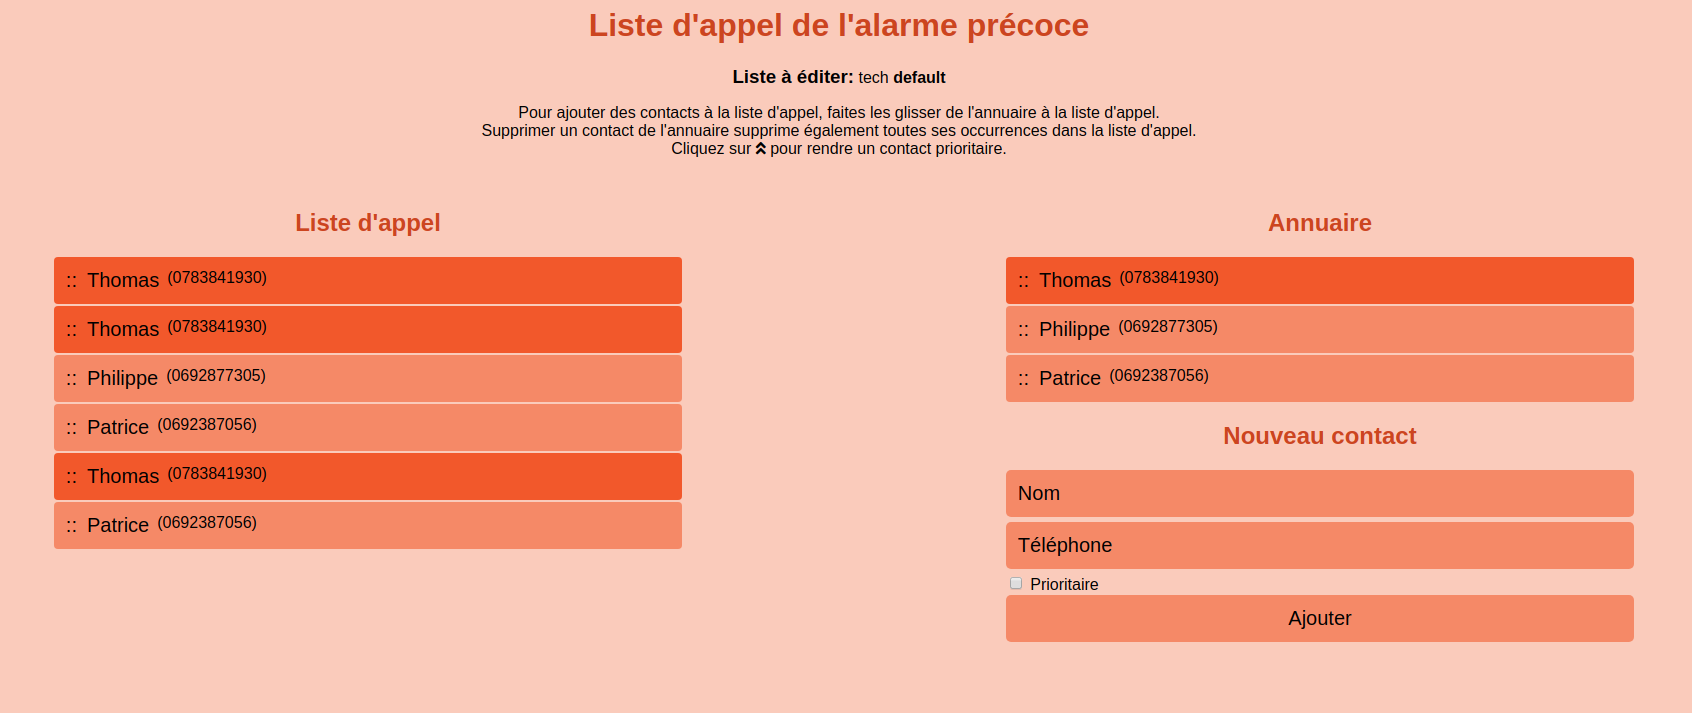
\includegraphics[width=\linewidth]{Illustrations/Interface_Appels.png}
      \caption{Capture d'écran de l'interface d'édition de listes d'appel}
      \label{fig:interface_web}
    \end{figure}
\end{center}

\subsection{Introduction}

L'interface Web se décompose en deux colonnes. 

La colonne de gauche correspond à la liste d'appel, à savoir quelles sont les personnes à appeler et dans quel ordre. Les éléments en couleur plus foncée correspondent au contact prioritaire. Ainsi, le premier élément est toujours de couleur foncée.

La colonne de droite se décompose en deux parties :

\begin{description}
    \item[L'annuaire] contient toutes les personnes connues du fichier ; on peut les y supprimer ou y définir le contact prioritaire ;
    \item[Le formulaire d'ajout de contact] permet d'ajouter un nouveau contact au fichier.
\end{description}

Pour ajouter un contact à la liste d'appel, il suffit de faire glisser le contact correspondant de la liste de droite à celle de gauche, à la position souhaitée.

Pour modifier l'ordre d'appel, on peut directement réordonner (en les faisant glisser) les éléments de la liste de gauche.

\subsection{Ajout d'un contact}

L'ajout d'un contact à la liste d'appels se fait de la façon suivante :

\begin{itemize}
    \item Remplir les champs \emph{Nom} et \emph{Téléphone} ;
    \item Cocher au besoin la case \emph{Prioritaire} ;
    \item Valider avec le bouton \emph{Valider}.
\end{itemize}

\paragraph{Case \emph{Prioritaire}\\}

La case \emph{Prioritaire} permet de définir un contact comme étant \emph{prioritaire}. Cela signifie que le premier de la liste d'appel sera \emph{toujours} celui-ci.\\
Un contact prioritaire peut se trouver à plusieurs endroits dans la liste d'appels, mais le premier élément sera toujours un contact prioritaire (si la liste d'appel contient un contact prioritaire). \\
Un seul contact peut être prioritaire à la fois.

\begin{center}
    \begin{figure}[ht]
      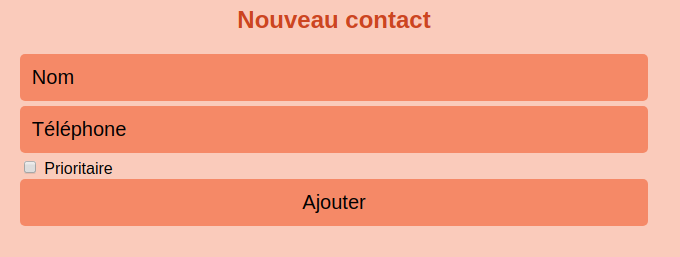
\includegraphics[width=\linewidth]{Illustrations/Nouveau_Contact.png}
      \caption{Formulaire de création de contact}
      \label{fig:creation_contact}
    \end{figure}
\end{center}

\subsection{Désactivation d'un contact}

Pour désactiver un contact (ou, s'il est présent plusieurs fois dans la liste d'appel, supprimer une de ses occurrences), utiliser la croix qui apparaît à gauche de l'élément lorsque l'on passe le pointeur de la souris sur l'élément dans la liste d'appel (à droite).\\

\emph{Vous ne pouvez pas supprimer tous les contacts de la liste d'appel.}

\subsection{Suppression d'un contact}

Pour supprimer un contact de la liste d'appel, utiliser la croix qui apparaît à gauche de l'élément correspondant dans la liste des contacts disponibles (à gauche). \\
\emph{Supprimer un contact supprime également toutes ses occurrences dans la liste d'appel.}


\subsection{Réglage du contact prioritaire}

Pour définir le contact prioritaire, utiliser le bouton avec les deux flèches vers le haut qui apparaît au passage de la souris dans l'annuaire. 

Une nouvelle entrée sera alors automatiquement ajoutée à la liste d'appel pour que le nouveau contact prioritaire soit présent en haut.

\begin{center}
    \begin{figure}[h!]
      
\includegraphics[width=\linewidth]{Illustrations/Contact_Prioritaire.png}
      \caption{Définition du contact prioritaire}
      \label{fig:contact_prioritaire}
    \end{figure}
\end{center}
\end{document}
